% BEAMER ----
% This is just here so I know exactly what I'm looking at in Rstudio when messing with stuff.
\documentclass[10pt,ignorenonframetext,,aspectratio=149]{beamer}
\usetheme{metropolis}
\usefonttheme{serif} % use mainfont rather than sansfont for slide text
\setbeamertemplate{caption}[numbered]
\setbeamertemplate{caption label separator}{: }
\setbeamercolor{caption name}{fg=normal text.fg}
\usepackage{lmodern}
\usepackage{amssymb,amsmath}
\usepackage{ifxetex,ifluatex}
\usepackage{fixltx2e} % provides \textsubscript
\ifnum 0\ifxetex 1\fi\ifluatex 1\fi=0 % if pdftex
  \usepackage[T1]{fontenc}
  \usepackage[utf8]{inputenc}
\else % if luatex or xelatex
  \ifxetex
    \usepackage{mathspec}
  \else
    \usepackage{fontspec}
  \fi
  \defaultfontfeatures{Ligatures=TeX,Scale=MatchLowercase}
  \newcommand{\euro}{€}
    \setmainfont[]{Open Sans Light}
\fi
% use upquote if available, for straight quotes in verbatim environments
\IfFileExists{upquote.sty}{\usepackage{upquote}}{}
% use microtype if available
\IfFileExists{microtype.sty}{%
\usepackage{microtype}
\UseMicrotypeSet[protrusion]{basicmath} % disable protrusion for tt fonts
}{}

% --------------------------------
% Separating this because this no
% longer works as of pandoc 3.2.1
% -------------------------------
%%\usepackage{graphicx,grffile}
%\makeatletter
%\def\maxwidth{\ifdim\Gin@nat@width>\linewidth\linewidth\else\Gin@nat@width\fi}
%\def\maxheight{\ifdim\Gin@nat@height>\textheight0.8\textheight\else\Gin@nat@height\fi}
%\makeatother
%% Scale images if necessary, so that they will not overflow the page
%% margins by default, and it is still possible to overwrite the defaults
%% using explicit options in \includegraphics[width, height, ...]{}
%\setkeys{Gin}{width=\maxwidth,height=\maxheight,keepaspectratio}
%
% ---------------------------------
% This works now: HT: Justin Esarey
% ---------------------------------
\usepackage{graphicx}
\makeatletter
\newsavebox\pandoc@box
\newcommand*\pandocbounded[1]{% scales image to fit in text height/width
  \sbox\pandoc@box{#1}%
  \Gscale@div\@tempa{\textheight}{\dimexpr\ht\pandoc@box+\dp\pandoc@box\relax}%
  \Gscale@div\@tempb{\linewidth}{\wd\pandoc@box}%
  \ifdim\@tempb\p@<\@tempa\p@\let\@tempa\@tempb\fi% select the smaller of both
  \ifdim\@tempa\p@<\p@\scalebox{\@tempa}{\usebox\pandoc@box}%
  \else\usebox{\pandoc@box}%
  \fi%
}
% Set default figure placement to htbp
\def\fps@figure{htbp}
\makeatother

% ^ saving this note in case I want some kind of conditional operation thingie.


% Comment these out if you don't want a slide with just the
% part/section/subsection/subsubsection title:
\AtBeginPart{
  \let\insertpartnumber\relax
  \let\partname\relax
  \frame{\partpage}
}
\AtBeginSection{
  \let\insertsectionnumber\relax
  \let\sectionname\relax
  \frame{\sectionpage}
}
\AtBeginSubsection{
  \let\insertsubsectionnumber\relax
  \let\subsectionname\relax
  \frame{\subsectionpage}
}

\setlength{\emergencystretch}{3em}  % prevent overfull lines
\providecommand{\tightlist}{%
  \setlength{\itemsep}{0pt}\setlength{\parskip}{0pt}}
\setcounter{secnumdepth}{0}

\title{The Linear Model and OLS}
\subtitle{IRIII.2 -- Quantitative Methods in the Study of International
Relations}
\author{Steven V. Miller}
\date{}


%% Here's everything I added.
%%--------------------------

\usepackage{graphicx}
\usepackage{rotating}
%\setbeamertemplate{caption}[numbered]
\usepackage{hyperref}
\usepackage{caption}
\usepackage[normalem]{ulem}
%\mode<presentation>
\usepackage{wasysym}
%\usepackage{amsmath}


% Get rid of navigation symbols.
%-------------------------------
\setbeamertemplate{navigation symbols}{}

% Optional institute tags and titlegraphic.
% Do feel free to change the titlegraphic if you don't want it as a Markdown field.
%----------------------------------------------------------------------------------
\institute{Department of Economic History and International Relations}

% \titlegraphic{\includegraphics[width=0.3\paperwidth]{\string~/Dropbox/teaching/clemson-academic.png}} % <-- if you want to know what this looks like without it as a Markdown field.
% -----------------------------------------------------------------------------------------------------
\titlegraphic{\vspace{6cm}\includegraphics[width=0.3\paperwidth]{/home/steve/Koofr/su/su-logotyp.png}}


% Some additional title page adjustments.
%----------------------------------------
\setbeamertemplate{title page}[empty]
%\date{}
\setbeamerfont{subtitle}{size=\small}

\setbeamercovered{transparent}

% Some optional colors. Change or add as you see fit.
%---------------------------------------------------
\definecolor{clemsonpurple}{HTML}{522D80}
 \definecolor{clemsonorange}{HTML}{F66733}
\definecolor{uiucblue}{HTML}{003C7D}
\definecolor{uiucorange}{HTML}{F47F24}

% new gig just dropped
\definecolor{sublue}{HTML}{002F5F}
\definecolor{susky}{HTML}{ACDEE6}
\definecolor{suwater}{HTML}{9BB2CE}





% Some optional color adjustments to Beamer. Change as you see fit.
%------------------------------------------------------------------
\setbeamercolor{frametitle}{fg=sublue,bg=white}
\setbeamercolor{title}{fg=sublue,,bg=white}
\setbeamercolor{local structure}{fg=sublue,}
\setbeamercolor{section in toc}{fg=sublue,bg=white}
% \setbeamercolor{subsection in toc}{fg=clemsonorange,bg=white}
\setbeamercolor{footline}{fg=sublue!50, bg=white}
\setbeamercolor{block title}{fg=sublue,bg=white}
\setbeamercolor{background canvas}{bg=white}


\setbeamercolor{title separator}{fg=suwater}

\let\Tiny=\tiny


% Sections and subsections should not get their own damn slide.
%--------------------------------------------------------------
\AtBeginPart{}
\AtBeginSection{}
\AtBeginSubsection{}
\AtBeginSubsubsection{}

% Suppress some of Markdown's weird default vertical spacing.
%------------------------------------------------------------
\setlength{\emergencystretch}{0em}  % prevent overfull lines
\setlength{\parskip}{0pt}


% Allow for those simple two-tone footlines I like.
% Edit the colors as you see fit.
%--------------------------------------------------
\defbeamertemplate*{footline}{my footline}{%
    \ifnum\insertpagenumber=1
    \hbox{%
        \begin{beamercolorbox}[wd=\paperwidth,ht=.8ex,dp=1ex,center]{}%
      % empty environment to raise height
        \end{beamercolorbox}%
    }%
    \vskip0pt%
    \else%
        \Tiny{%
            \hfill%
		\vspace*{1pt}%
            \insertframenumber/\inserttotalframenumber \hspace*{0.1cm}%
            \newline%
            \color{sublue}{\rule{\paperwidth}{0.4mm}}\newline%
            \color{suwater}{\rule{\paperwidth}{.4mm}}%
        }%
    \fi%
}

% Various cosmetic things, though I must confess I forget what exactly these do and why I included them.
%-------------------------------------------------------------------------------------------------------
\setbeamercolor{structure}{fg=blue}
\setbeamercolor{local structure}{parent=structure}
\setbeamercolor{item projected}{parent=item,use=item,fg=sublue,bg=white}
\setbeamercolor{enumerate item}{parent=item}

% Adjust some item elements. More cosmetic things.
%-------------------------------------------------
\setbeamertemplate{itemize item}{\color{sublue}$\bullet$}
\setbeamertemplate{itemize subitem}{\color{sublue}\scriptsize{$\bullet$}}
\setbeamertemplate{itemize/enumerate body end}{\vspace{.6\baselineskip}} % So I'm less inclined to use \medskip and \bigskip in Markdown.

% Automatically center images
% ---------------------------
% Note: this is for ![](image.png) images
% Use "fig.align = "center" for R chunks

\usepackage{etoolbox}

\AtBeginDocument{%
  \letcs\oig{@orig\string\includegraphics}%
  \renewcommand<>\includegraphics[2][]{%
    \only#3{%
      {\centering\oig[{#1}]{#2}\par}%
    }%
  }%
}

% I think I've moved to xelatex now. Here's some stuff for that.
% --------------------------------------------------------------
% I could customize/generalize this more but the truth is it works for my circumstances.

\ifxetex
\setbeamerfont{title}{family=\fontspec{Titillium Web}}
\setbeamerfont{frametitle}{family=\fontspec{Titillium Web}}
% Commented out -----
%\setbeamerfont{title}{family=\fontspec{Titillium Web}}
%\setbeamerfont{frametitle}{family=\fontspec{Titillium Web}}
\usepackage[font=small,skip=0pt]{caption}
 \else
 \fi

% {modelsummary} and {kableExtra} support
% --------------------------------------------------------------
% Rather than clutter my preambles for this stuff, it's just going to come by default.
\usepackage{dcolumn}
\usepackage{booktabs}
\usepackage{longtable}
\usepackage{array}
\usepackage{multirow}
\usepackage{wrapfig}
\usepackage{float}
\usepackage{colortbl}
\usepackage{pdflscape}
\usepackage{tabu}
\usepackage{threeparttable}


% Some random stuff now...
% ------------------------

\usepackage{tikz}

\newcommand{\shrug}[1][]{%
\begin{tikzpicture}[baseline,x=0.8\ht\strutbox,y=0.8\ht\strutbox,line width=0.125ex,#1]
\def\arm{(-2.5,0.95) to (-2,0.95) (-1.9,1) to (-1.5,0) (-1.35,0) to (-0.8,0)};
\draw \arm;
\draw[xscale=-1] \arm;
\def\headpart{(0.6,0) arc[start angle=-40, end angle=40,x radius=0.6,y radius=0.8]};
\draw \headpart;
\draw[xscale=-1] \headpart;
\def\eye{(-0.075,0.15) .. controls (0.02,0) .. (0.075,-0.15)};
\draw[shift={(-0.3,0.8)}] \eye;
\draw[shift={(0,0.85)}] \eye;
% draw mouth
\draw (-0.1,0.2) to [out=15,in=-100] (0.4,0.95);
\end{tikzpicture}}

% cols environment, for column-hackery.

\newenvironment{cols}[1][]{}{}

\newenvironment{col}[1]{\begin{minipage}{#1}\ignorespaces}{%
\end{minipage}
\ifhmode\unskip\fi
\aftergroup\useignorespacesandallpars}

\def\useignorespacesandallpars#1\ignorespaces\fi{%
#1\fi\ignorespacesandallpars}

\makeatletter
\def\ignorespacesandallpars{%
  \@ifnextchar\par
    {\expandafter\ignorespacesandallpars\@gobble}%
    {}%
}
\makeatother


% header includes go last.

\usepackage{dcolumn}
\usepackage{booktabs}
\usepackage{longtable}
\usepackage{array}
\usepackage{multirow}
\usepackage{wrapfig}
\usepackage{float}
\usepackage{colortbl}
\usepackage{pdflscape}
\usepackage{tabu}
\usepackage{threeparttable}
\usepackage{booktabs}
\usepackage{longtable}
\usepackage{array}
\usepackage{multirow}
\usepackage{wrapfig}
\usepackage{float}
\usepackage{colortbl}
\usepackage{pdflscape}
\usepackage{tabu}
\usepackage{threeparttable}
\usepackage{threeparttablex}
\usepackage[normalem]{ulem}
\usepackage{makecell}
\usepackage{xcolor}

% Okay, and begin the actual document...

\begin{document}
\frame{\titlepage}

\section{Introduction}\label{introduction}

\begin{frame}{Goal(s) for Today}
\phantomsection\label{goals-for-today}
\begin{enumerate}
\tightlist
\item
  Introduce the basic intuition behind linear regression.
\item
  Give an applied example and unpack it.
\end{enumerate}
\end{frame}

\begin{frame}{Elsewhere on My Blog}
\phantomsection\label{elsewhere-on-my-blog}
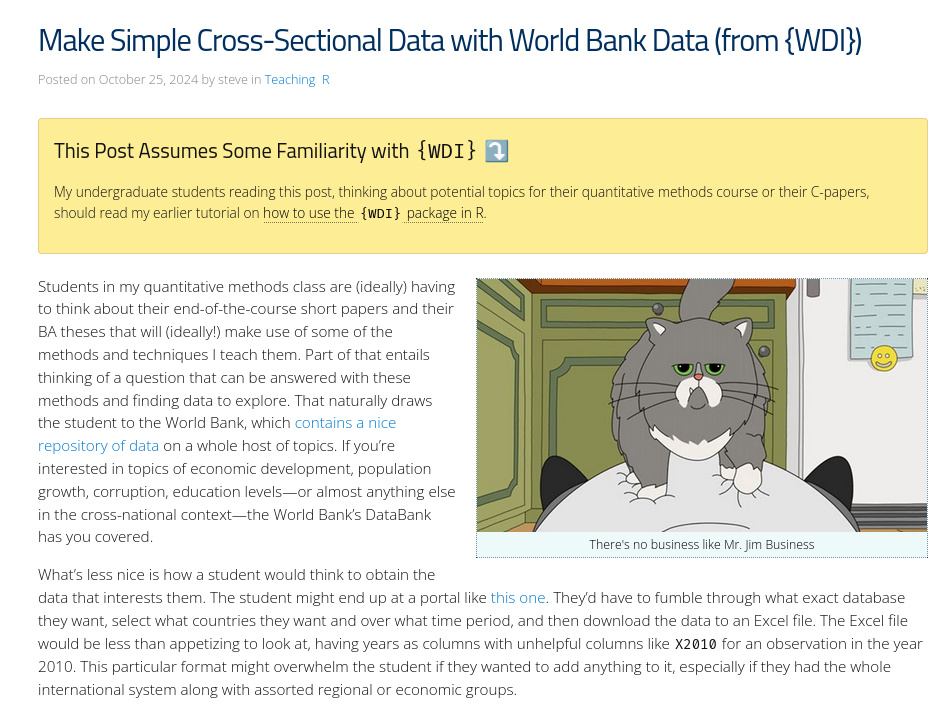
\includegraphics[width=0.8\linewidth,height=\textheight,keepaspectratio]{mr-jim.png}
\end{frame}

\begin{frame}{Elsewhere on My Blog}
\phantomsection\label{elsewhere-on-my-blog-1}
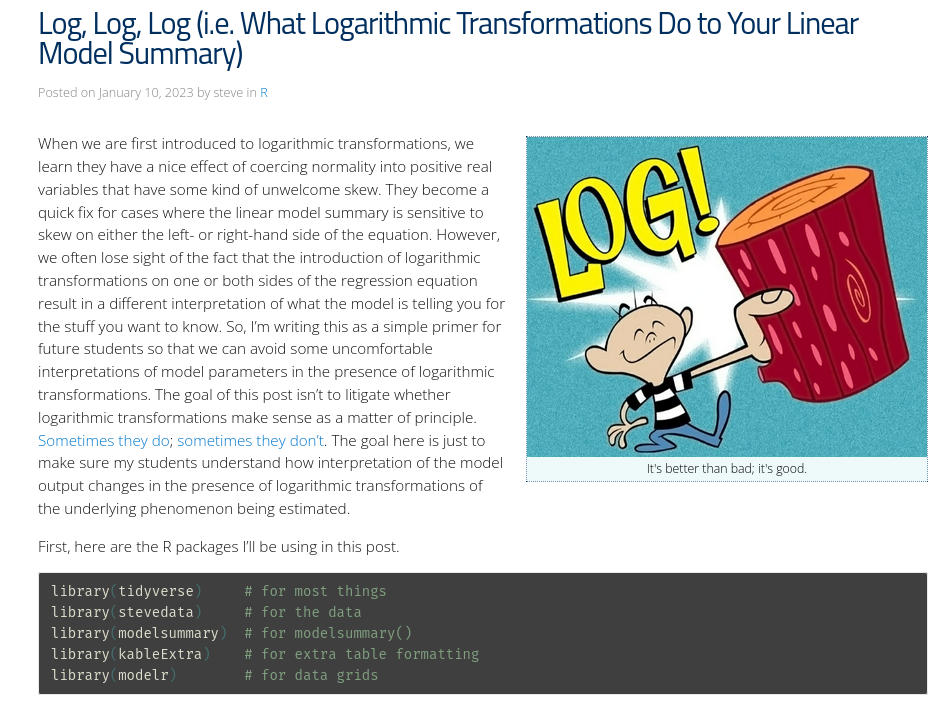
\includegraphics[width=0.8\linewidth,height=\textheight,keepaspectratio]{log-log-log.png}
\end{frame}

\section{The Linear Model and OLS}\label{the-linear-model-and-ols}

\subsection{Demystifying, with the
Quickness}\label{demystifying-with-the-quickness}

\begin{frame}{Correlation to Linear Regression}
\phantomsection\label{correlation-to-linear-regression}
Correlation has a lot of nice properties.

\begin{itemize}
\tightlist
\item
  It's another ``first step'' analytical tool.
\item
  Useful for detecting \textbf{multicollinearity}.

  \begin{itemize}
  \tightlist
  \item
    This is when two independent variables correlate so highly that no
    partial effect for either can be summarized.
  \end{itemize}
\end{itemize}

However, it's neutral on what is \emph{x} and what is \emph{y}.

\begin{itemize}
\tightlist
\item
  It won't communicate cause and effect.
\end{itemize}

Fortunately, regression can do that for us (under ideal conditions).
\end{frame}

\begin{frame}{Demystifying Regression}
\phantomsection\label{demystifying-regression}
Does this look familiar?

\[
y = mx + b
\]
\end{frame}

\begin{frame}{Demystifying Regression}
\phantomsection\label{demystifying-regression-1}
That was the slope-intercept equation.

\begin{itemize}
\tightlist
\item
  \emph{b} is the intercept: the observed \emph{y} when \emph{x} = 0.
\item
  \emph{m} is the familiar ``rise over run'', measuring the amount of
  change in \emph{y} for a unit change in \emph{x}.
\end{itemize}
\end{frame}

\begin{frame}{Demystifying Regression}
\phantomsection\label{demystifying-regression-2}
The slope-intercept equation is, in essence, the representation of a
regression line.

\begin{itemize}
\tightlist
\item
  However, statisticians prefer a different rendering of the same
  concept measuring linear change.
\end{itemize}

\[
y = a + b(x)
\]

The \emph{b} is the \textbf{regression coefficient} that communicates
the change in \emph{y} for each unit change in \emph{x}.

\begin{itemize}
\tightlist
\item
  However, this is a deterministic function. We live in a stochastic
  world.
\end{itemize}
\end{frame}

\begin{frame}{A Full Statement of the Regression Formula}
\phantomsection\label{a-full-statement-of-the-regression-formula}
If you've followed that, we're just going to add two more things:

\[
\hat{y} = \hat{a} + \hat{b}(x) + e
\]

\ldots where:

\begin{itemize}
\tightlist
\item
  \(\hat{y}\), \(\hat{a}\) and \(\hat{b}\) are estimates of \emph{y},
  \emph{a}, and \emph{b} over the data.
\item
  \emph{e} is the error term.

  \begin{itemize}
  \tightlist
  \item
    It contains random sampling error, prediction error, and predictors
    not included in the model.
  \end{itemize}
\end{itemize}

We can further extend this out by including more \emph{x} variables into
our equation.

\begin{itemize}
\tightlist
\item
  Mechanically: there's a lot to unpack. Conceptually: not really (at
  this level).
\end{itemize}
\end{frame}

\begin{frame}{Getting a Regression Coefficient}
\phantomsection\label{getting-a-regression-coefficient}
How do we get a regression coefficient for more complicated data?

\begin{itemize}
\tightlist
\item
  Start with the \textbf{prediction error}, formally: \(y_i - \hat{y}\).
\item
  Square them. In other words: \((y_i - \hat{y})^2\)

  \begin{itemize}
  \tightlist
  \item
    If you didn't, the sum of prediction errors would equal zero.
  \end{itemize}
\end{itemize}

The regression coefficient that emerges minimizes the sum of squared
differences (\((y_i - \hat{y})^2\)).

\begin{itemize}
\tightlist
\item
  Put another way: ``ordinary least squares'' (OLS) regression.
\end{itemize}
\end{frame}

\subsection{An Applied Example: The Correlates of
Tourism}\label{an-applied-example-the-correlates-of-tourism}

\begin{frame}{An Applied Example: The Correlates of Tourism}
\phantomsection\label{an-applied-example-the-correlates-of-tourism-1}
\begin{figure}
\centering
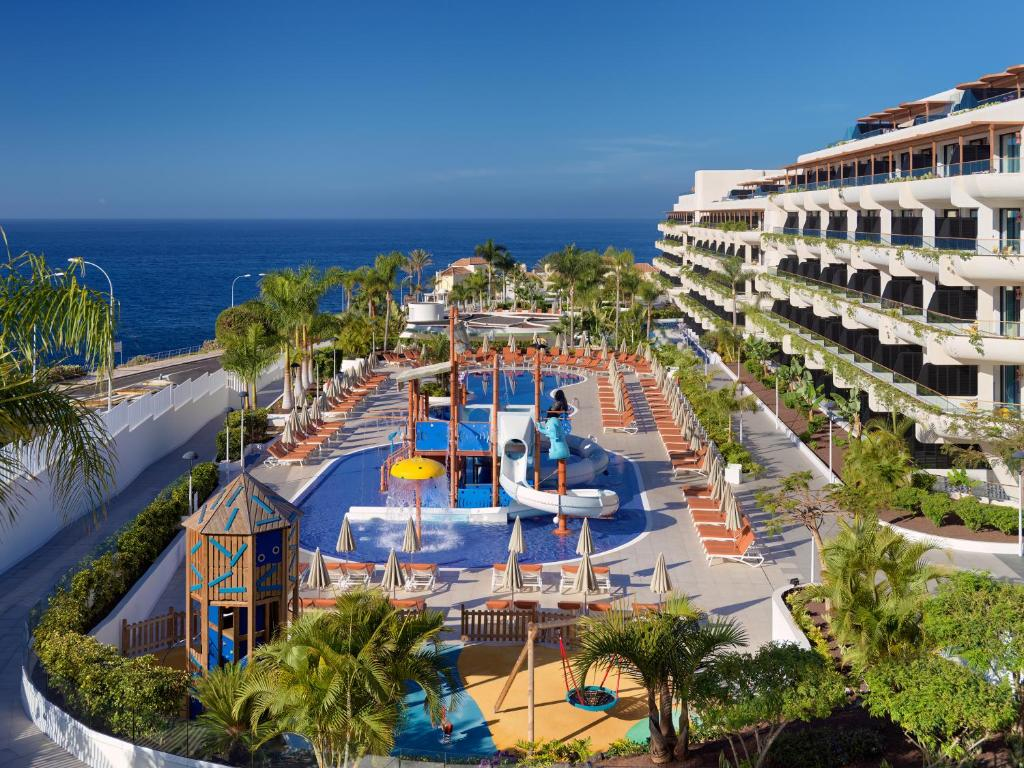
\includegraphics[width=0.8\linewidth,height=\textheight,keepaspectratio]{ci-hotel.jpg}
\caption{I'll be honest that a trip to the Canaries sounds mighty nice
in February\ldots{}}
\end{figure}
\end{frame}

\begin{frame}{An Applied Example: The Correlates of Tourism}
\phantomsection\label{an-applied-example-the-correlates-of-tourism-2}
Academic interest in the international relations/IPE of tourism may owe
to H.P. Gray (1966).

\begin{itemize}
\tightlist
\item
  Tourism as a form of ``soft power'' projection.

  \begin{itemize}
  \tightlist
  \item
    (i.e.~you've seen the YouTube ads for Türkiye or Arsenal's ``Visit
    Rwanda'' patch)
  \end{itemize}
\item
  Tourism-dependent countries have \emph{a lot} of subtle risks.

  \begin{itemize}
  \tightlist
  \item
    Behave like rentier states; economy is dependent on foreign
    receipts.
  \item
    Environmental sustainability concerns are paramount.
  \item
    \emph{Very} sensitive to massive shocks like the pandemic or
    political violence.
  \end{itemize}
\end{itemize}

Thus, tourism is a kind of barometer or measuring stick for important
questions of development and peace.

\begin{itemize}
\tightlist
\item
  \emph{ed.~notice how I'm selling you on the value of doing this in the
  first place\ldots{}}
\end{itemize}
\end{frame}

\begin{frame}[fragile]{A Simple Exercise}
\phantomsection\label{a-simple-exercise}
I gathered data from the World Bank's repository for a simple
cross-sectional exercise.

\begin{itemize}
\tightlist
\item
  \emph{DV}: number of arrivals for international tourism (logged)
\item
  \emph{IVs}: conceptually (operationally)
  \texttt{{[}expected\ effect{]}}

  \begin{itemize}
  \tightlist
  \item
    Ease of access/infrastructure for visitors (passengers carried by
    air transport, logged) \texttt{{[}+{]}}
  \item
    Relative price to USD (price level ratio of PPP to market exchange
    rate) \texttt{{[}-{]}}
  \item
    Economic development (GDP per capita, logged) \texttt{{[}+{]}}
  \item
    Political security (political stability/absence of violence,
    terrorism) \texttt{{[}+{]}}
  \item
    Dummy variable for ``fragile/conflict affected states (FCAS)''
    \texttt{{[}-{]}}
  \end{itemize}
\end{itemize}

I use the same lag and group-by fill I describe in the blog post I
reference earlier.

\begin{itemize}
\tightlist
\item
  Referent year: 2019 (or shortly before it)
\end{itemize}
\end{frame}

\begin{frame}{The Model(s)}
\phantomsection\label{the-models}
We'll run two linear models.

\begin{enumerate}
\tightlist
\item
  Bivariate model with just relative price.
\item
  Full model with all the other stuff.
\end{enumerate}
\end{frame}

\begin{frame}{}
\phantomsection\label{section}
\pandocbounded{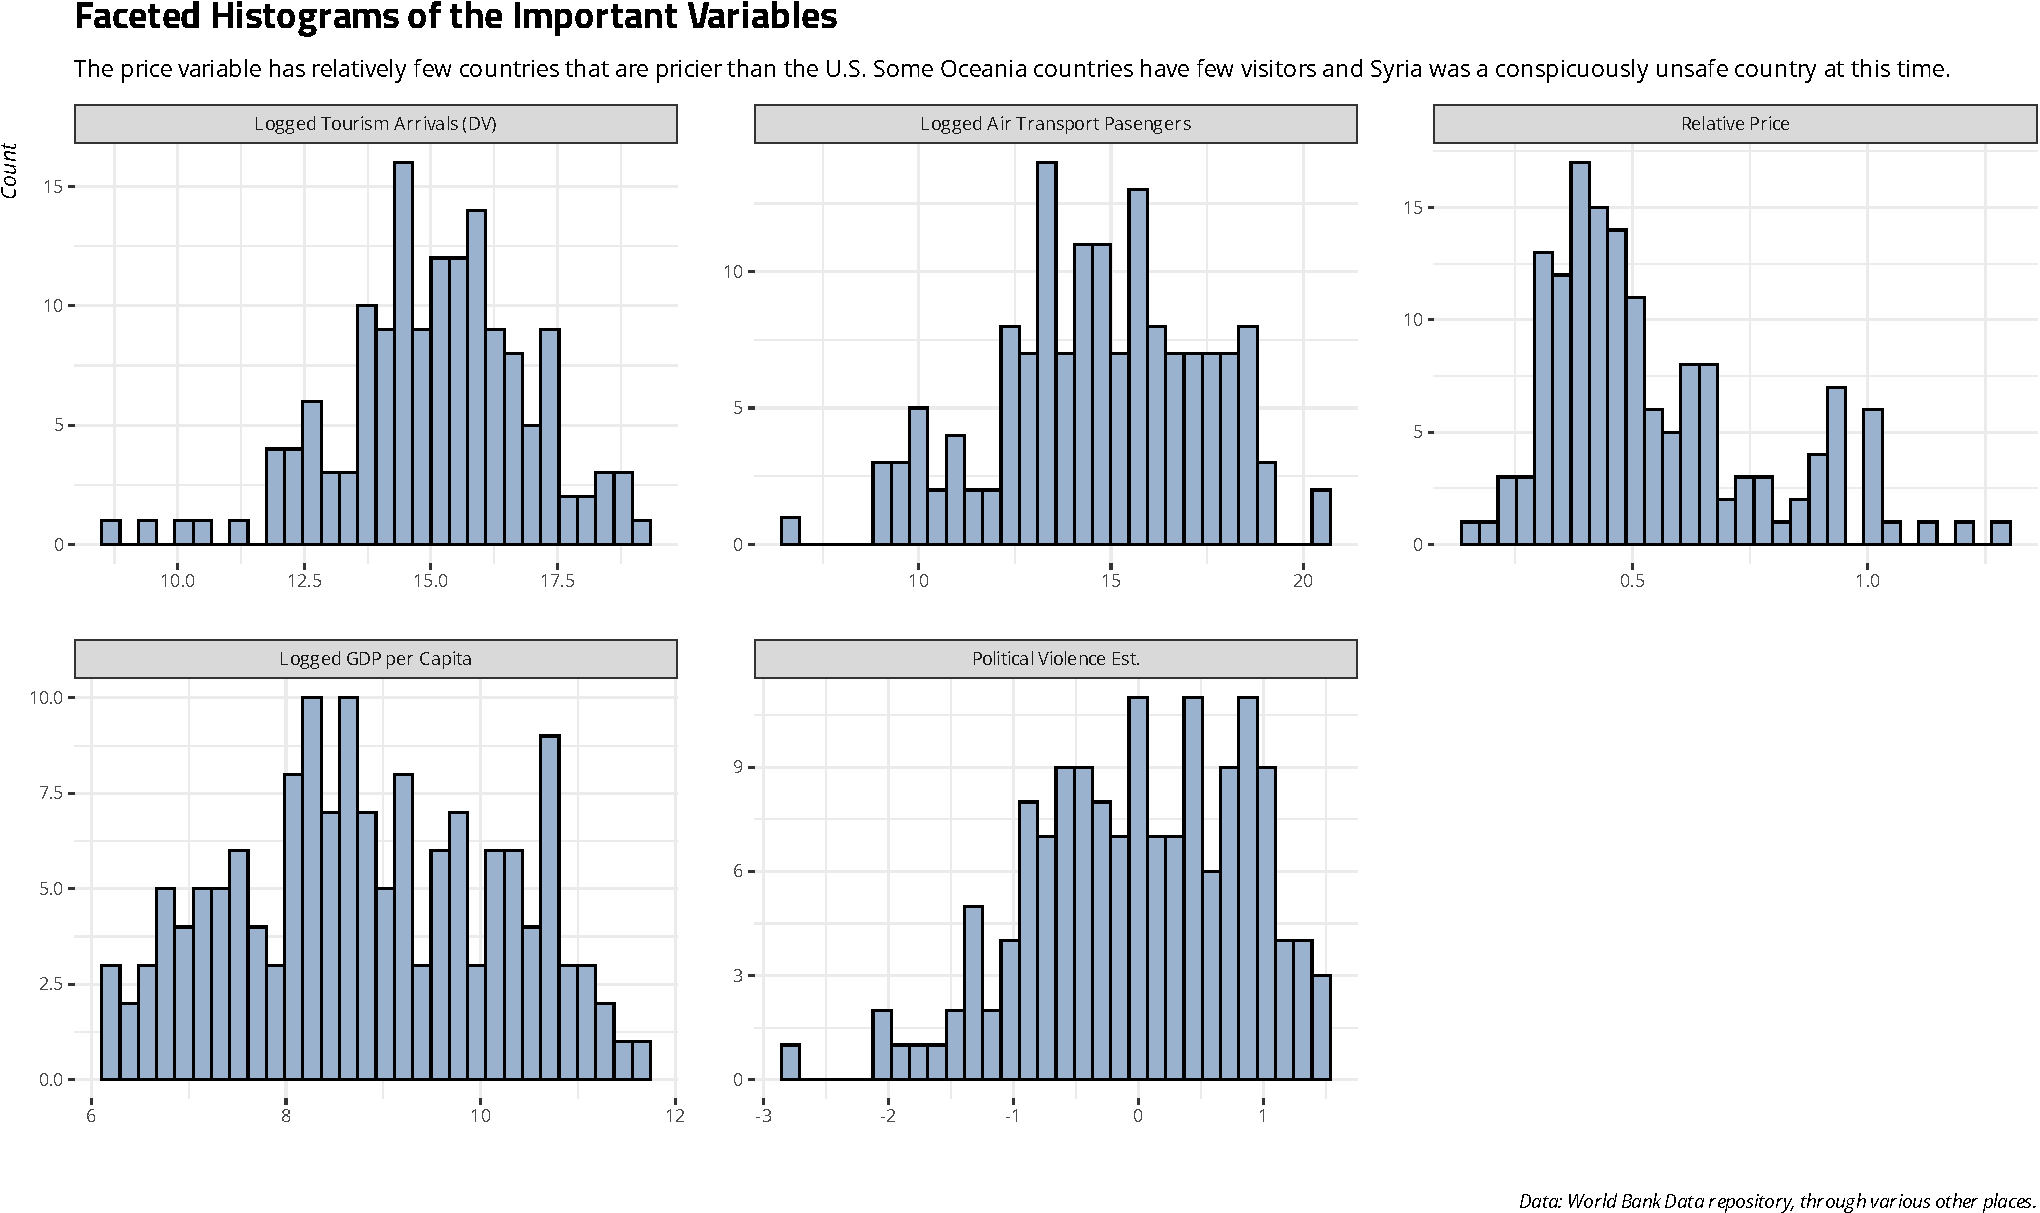
\includegraphics[keepaspectratio]{figs/unnamed-chunk-1.pdf}}
\end{frame}

\begin{frame}{}
\phantomsection\label{section-1}
\pandocbounded{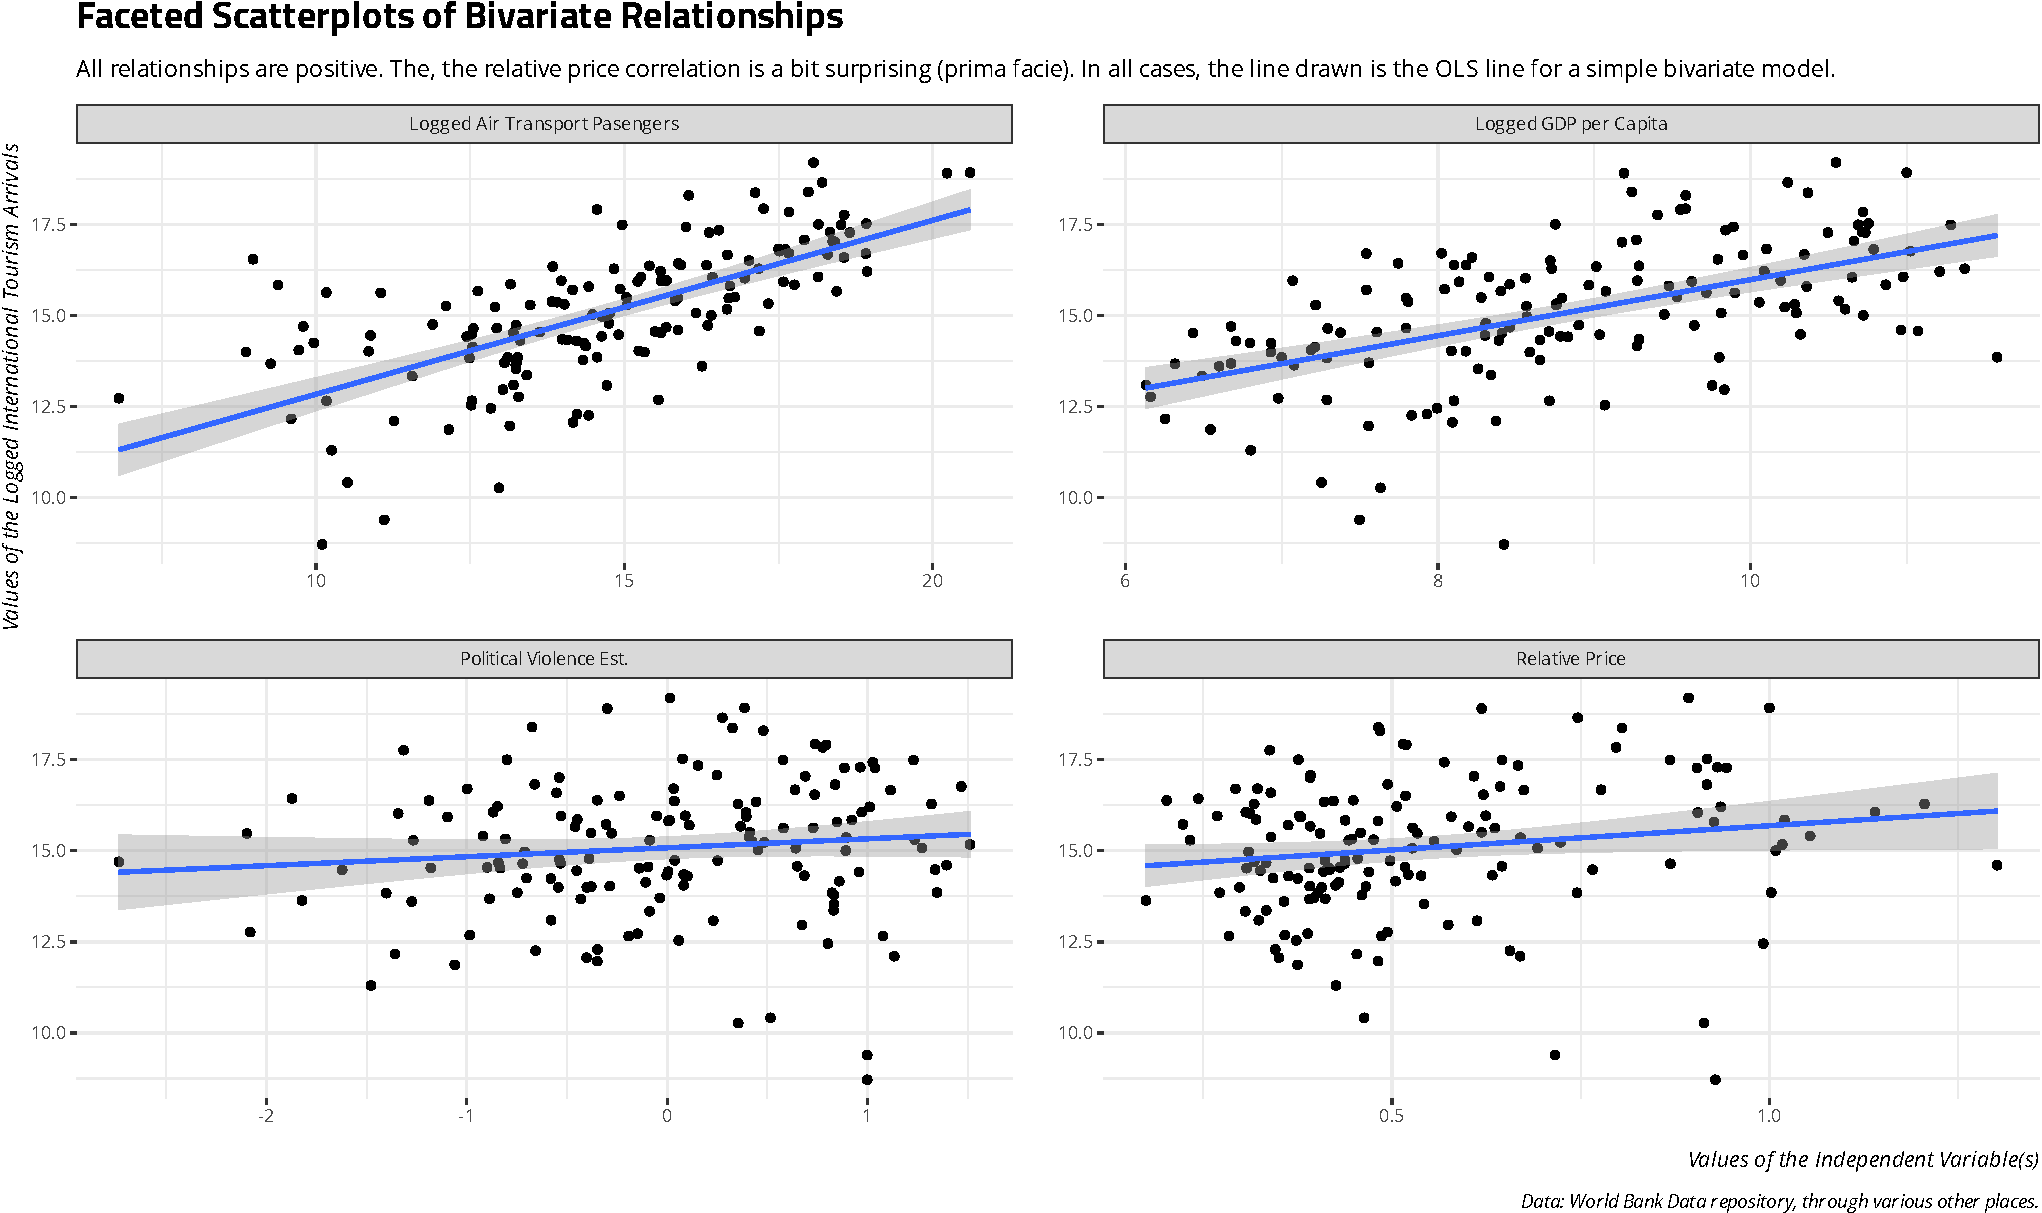
\includegraphics[keepaspectratio]{figs/unnamed-chunk-2.pdf}}
\end{frame}

\begin{frame}{}
\phantomsection\label{section-2}
\begin{table}
\centering\centering
\caption{\label{tab:unnamed-chunk-3}Cross-National Correlates of (Logged) International Tourism Arrivals}
\centering
\fontsize{6}{8}\selectfont
\begin{tabular}[t]{lcc}
\toprule
\textbf{ } & \textbf{Bivariate} & \textbf{Full Model}\\
\midrule
Relative Price & 1.333* & -1.565*\\
 & (0.664) & (0.671)\\
Air Transport Passengers (Logged) &  & 0.283***\\
 &  & (0.047)\\
GDP per Capita (Logged) &  & 0.763***\\
 &  & (0.136)\\
Political Stability &  & -0.631***\\
 &  & (0.182)\\
Fragile/Conflict-Affected State &  & -1.360***\\
 &  & (0.366)\\
Intercept & 14.358*** & 5.216***\\
 & (0.392) & (0.911)\\
\midrule
Num.Obs. & 149 & 149\\
R2 & 0.027 & 0.627\\
R2 Adj. & 0.020 & 0.614\\
F & 4.026 & 48.172\\
\bottomrule
\multicolumn{3}{l}{\rule{0pt}{1em}+ p $<$ 0.1, * p $<$ 0.05, ** p $<$ 0.01, *** p $<$ 0.001}\\
\end{tabular}
\end{table}
\end{frame}

\begin{frame}{}
\phantomsection\label{section-3}

\includegraphics[width=0.8\linewidth,height=\textheight,keepaspectratio]{dawson_crying.jpg}
\end{frame}

\subsection{How to Interpret Regression
Output}\label{how-to-interpret-regression-output}

\begin{frame}{How to Interpret a Regression Table Like This}
\phantomsection\label{how-to-interpret-a-regression-table-like-this}
\begin{enumerate}
\tightlist
\item
  Find the variable(s) of interest.
\item
  Look for direction (positive/negative)
\item
  Look for ``stars'' (to determine statistical significance)
\end{enumerate}
\end{frame}

\begin{frame}{}
\phantomsection\label{section-4}
\begin{table}
\centering\centering
\caption{\label{tab:unnamed-chunk-4}Cross-National Correlates of (Logged) International Tourism Arrivals}
\centering
\fontsize{6}{8}\selectfont
\begin{tabular}[t]{>{}l>{}cc}
\toprule
\textbf{ } & \textbf{Bivariate} & \textbf{Full Model}\\
\midrule
\cellcolor[HTML]{ffffff}{\textcolor[HTML]{000000}{\textbf{Relative Price}}} & \cellcolor[HTML]{00cc00}{\textcolor[HTML]{ffffff}{\textbf{1.333*}}} & \cellcolor[HTML]{cc0000}{\textcolor[HTML]{ffffff}{\textbf{-1.565*}}}\\
\cellcolor[HTML]{ffffff}{\textcolor[HTML]{000000}{\textbf{}}} & \cellcolor[HTML]{00cc00}{\textcolor[HTML]{ffffff}{\textbf{(0.664)}}} & \cellcolor[HTML]{cc0000}{\textcolor[HTML]{ffffff}{\textbf{(0.671)}}}\\
\cellcolor[HTML]{ffffff}{\textcolor[HTML]{000000}{\textbf{\textbf{Air Transport Passengers (Logged)}}}} & \cellcolor[HTML]{00cc00}{\textcolor[HTML]{ffffff}{\textbf{\textbf{}}}} & \cellcolor[HTML]{00cc00}{\textcolor[HTML]{ffffff}{\textbf{\textbf{0.283***}}}}\\
\cellcolor[HTML]{ffffff}{\textcolor[HTML]{000000}{\textbf{\textbf{}}}} & \cellcolor[HTML]{00cc00}{\textcolor[HTML]{ffffff}{\textbf{\textbf{}}}} & \cellcolor[HTML]{00cc00}{\textcolor[HTML]{ffffff}{\textbf{\textbf{(0.047)}}}}\\
\cellcolor[HTML]{ffffff}{\textcolor[HTML]{000000}{\textbf{\textbf{GDP per Capita (Logged)}}}} & \cellcolor[HTML]{00cc00}{\textcolor[HTML]{ffffff}{\textbf{\textbf{}}}} & \cellcolor[HTML]{00cc00}{\textcolor[HTML]{ffffff}{\textbf{\textbf{0.763***}}}}\\
\cellcolor[HTML]{ffffff}{\textcolor[HTML]{000000}{\textbf{\textbf{}}}} & \cellcolor[HTML]{00cc00}{\textcolor[HTML]{ffffff}{\textbf{\textbf{}}}} & \cellcolor[HTML]{00cc00}{\textcolor[HTML]{ffffff}{\textbf{\textbf{(0.136)}}}}\\
\cellcolor[HTML]{ffffff}{\textcolor[HTML]{000000}{\textbf{\textbf{Political Stability}}}} & \cellcolor[HTML]{cc0000}{\textcolor[HTML]{ffffff}{\textbf{\textbf{}}}} & \cellcolor[HTML]{cc0000}{\textcolor[HTML]{ffffff}{\textbf{\textbf{-0.631***}}}}\\
\cellcolor[HTML]{ffffff}{\textcolor[HTML]{000000}{\textbf{\textbf{}}}} & \cellcolor[HTML]{cc0000}{\textcolor[HTML]{ffffff}{\textbf{\textbf{}}}} & \cellcolor[HTML]{cc0000}{\textcolor[HTML]{ffffff}{\textbf{\textbf{(0.182)}}}}\\
\cellcolor[HTML]{ffffff}{\textcolor[HTML]{000000}{\textbf{\textbf{Fragile/Conflict-Affected State}}}} & \cellcolor[HTML]{cc0000}{\textcolor[HTML]{ffffff}{\textbf{\textbf{}}}} & \cellcolor[HTML]{cc0000}{\textcolor[HTML]{ffffff}{\textbf{\textbf{-1.360***}}}}\\
\cellcolor[HTML]{ffffff}{\textcolor[HTML]{000000}{\textbf{\textbf{}}}} & \cellcolor[HTML]{cc0000}{\textcolor[HTML]{ffffff}{\textbf{\textbf{}}}} & \cellcolor[HTML]{cc0000}{\textcolor[HTML]{ffffff}{\textbf{\textbf{(0.366)}}}}\\
\cellcolor[HTML]{ffffff}{\textcolor[HTML]{000000}{Intercept}} & \cellcolor[HTML]{ffffff}{14.358***} & \cellcolor[HTML]{ffffff}{5.216***}\\
\cellcolor[HTML]{ffffff}{\textcolor[HTML]{000000}{}} & \cellcolor[HTML]{ffffff}{(0.392)} & \cellcolor[HTML]{ffffff}{(0.911)}\\
\midrule
\cellcolor[HTML]{ffffff}{\textcolor[HTML]{000000}{Num.Obs.}} & \cellcolor[HTML]{ffffff}{149} & \cellcolor[HTML]{ffffff}{149}\\
\cellcolor[HTML]{ffffff}{\textcolor[HTML]{000000}{R2}} & \cellcolor[HTML]{ffffff}{0.027} & \cellcolor[HTML]{ffffff}{0.627}\\
\cellcolor[HTML]{ffffff}{\textcolor[HTML]{000000}{R2 Adj.}} & \cellcolor[HTML]{ffffff}{0.020} & \cellcolor[HTML]{ffffff}{0.614}\\
\cellcolor[HTML]{ffffff}{\textcolor[HTML]{000000}{F}} & \cellcolor[HTML]{ffffff}{4.026} & \cellcolor[HTML]{ffffff}{48.172}\\
\bottomrule
\multicolumn{3}{l}{\rule{0pt}{1em}+ p $<$ 0.1, * p $<$ 0.05, ** p $<$ 0.01, *** p $<$ 0.001}\\
\end{tabular}
\end{table}
\end{frame}

\begin{frame}{Being More Careful with Our Takeaways}
\phantomsection\label{being-more-careful-with-our-takeaways}
``Number goes (up/down); other number goes (up/down); has (no) stars''
is fine when you're getting started.

\begin{itemize}
\tightlist
\item
  But let's do more.
\end{itemize}

We need to be smart with how we communicate this.

\begin{itemize}
\tightlist
\item
  Our DV is log-transformed and so are a few of our IVs.
\end{itemize}

Our plan of attack:

\begin{enumerate}
\tightlist
\item
  Start with the two variables that are log-transformed.
\item
  Talk about the variables that aren't log-transformed.
\end{enumerate}
\end{frame}

\begin{frame}[fragile]{The DV and IV are Both Log-Transformed}
\phantomsection\label{the-dv-and-iv-are-both-log-transformed}
\emph{Air transport passengers}: a 1\% increase in IV coincides with
estimated .283\% increase in DV.

\begin{itemize}
\tightlist
\item
  Alternatively, less helpfully: a unit increase log(x) increases log(y)
  by an estimated .311.
\end{itemize}

\emph{GDP per capita}: a 1\% change in GDP per capita -\textgreater{}
.763\% change in tourism arrivals.

\begin{itemize}
\tightlist
\item
  Alternatively, with more precision: \texttt{(1.01\^{}(.763)-1)*100} =
  .762\% change in tourism arrivals for 1\% increase in GDP per capita.
\end{itemize}

\textbf{Be mindful of the percentages!}

\begin{itemize}
\tightlist
\item
  ``one percent change in \emph{x} -\textgreater{} estimated (regression
  coefficient)\% change in \emph{y}''
\end{itemize}
\end{frame}

\begin{frame}[fragile]{The DV is Log-Transformed, but the IVs are Not}
\phantomsection\label{the-dv-is-log-transformed-but-the-ivs-are-not}
\emph{Relative price} (Full): a change from 0 to 1 in relative price
-\textgreater{} est. -1.56\% decrease in tourism arrivals.

\begin{itemize}
\tightlist
\item
  Be mindful: 0 = conceptual extreme; 1 = same price level as the U.S.
\end{itemize}

\emph{Political stability}: a change from 0 to 1 in political stability
-\textgreater{} -.631\% change in tourism arrivals.

\begin{itemize}
\tightlist
\item
  Alternatively: \texttt{exp(-.631)} = .532. A one-unit change in
  stability multiplies expected tourism arrivals by .532.
\item
  This interpretation works the same way for relative price because it's
  not log-transformed.
\end{itemize}

\emph{FCAS}: Being a FCAS (e.g.~Sudan) versus not being one
(e.g.~Sweden) decreases est. international tourism arrivals by est.
1.36\%.

\bigskip

\textbf{Here: unit changes in x -\textgreater{} (regression
coefficient)\% changes in y}
\end{frame}

\subsection{The Intercept and Goodness of Fit
Notes}\label{the-intercept-and-goodness-of-fit-notes}

\begin{frame}{Dont' Read Much into the Intercept}
\phantomsection\label{dont-read-much-into-the-intercept}
Don't bother interpreting the intercept.

\begin{itemize}
\tightlist
\item
  Nominally, it tells you the estimated value of \emph{y} when
  \emph{everything} covariate is set to 0.
\item
  In our case: a country has no air passengers, is \emph{infinitely}
  cheaper than the U.S., has no logged GDP per capita, has basically a
  middle level of political security and is not a FCAS.
\end{itemize}

There are advanced things you can do here, but don't bother at this
stage.

\begin{itemize}
\tightlist
\item
  Just know what this is ultimately communicating.
\end{itemize}
\end{frame}

\begin{frame}{The Goodness of Fit Statistics}
\phantomsection\label{the-goodness-of-fit-statistics}
\textbf{R-square}: proportion of variation in \emph{y} accounted for in
the model.

\begin{itemize}
\tightlist
\item
  In the bivariate model, it's quite literally Pearson's \emph{r},
  squared.
\end{itemize}

\textbf{Adj. R-square}: Includes a downweight for more (redundant)
parameters.

\begin{itemize}
\tightlist
\item
  Consider this the ``default'' R-square for your linear model.
\item
  The more junk you have in the model, the greater the separation
  between it and R-square.
\end{itemize}

\textbf{F}: ``overall model fit'' against guessing the mean.

\begin{itemize}
\tightlist
\item
  I'm including this because it's in the output. You're free to ignore
  it.
\end{itemize}
\end{frame}

\subsection{Assumptions and
Diagnostics}\label{assumptions-and-diagnostics}

\begin{frame}[fragile]{Assumptions and Diagnostics}
\phantomsection\label{assumptions-and-diagnostics-1}
There are \emph{myriad} assumptions of OLS. The ones we impress on you:

\begin{itemize}
\tightlist
\item
  \texttt{L}: the outcome \emph{y} model is a ``l''inear (and additive)
  function of the regressors.
\item
  \texttt{I}: the error term is ``i''ndependent/not correlated across
  observations.
\item
  \texttt{N}: the error term is ``n''ormally distributed.
\item
  \texttt{E}: the error term has ``e''qual/constant variance (i.e.~no
  heteroskedasticity).
\end{itemize}

Let me bore you with \texttt{L} and \texttt{N} at this round.

\begin{itemize}
\tightlist
\item
  Save \texttt{E} for me tormenting you in the C-paper stage.
\item
  \texttt{I} will matter a great deal for more advanced uses
  (i.e.~MA-level).
\end{itemize}
\end{frame}

\begin{frame}[fragile]{Diagnostics You Should Run}
\phantomsection\label{diagnostics-you-should-run}
\begin{enumerate}
\tightlist
\item
  Fitted-residual plot (overall, and/or by regressor)

  \begin{itemize}
  \tightlist
  \item
    This is the most ``bang for your buck'' OLS diagnostic. You should
    always run it.
  \end{itemize}
\item
  Residual density plot (or QQ plot)

  \begin{itemize}
  \tightlist
  \item
    Useful for the \texttt{N} part, for as unimportant as that
    assumption mostly is.
  \end{itemize}
\end{enumerate}
\end{frame}

\begin{frame}{}
\phantomsection\label{section-5}
\pandocbounded{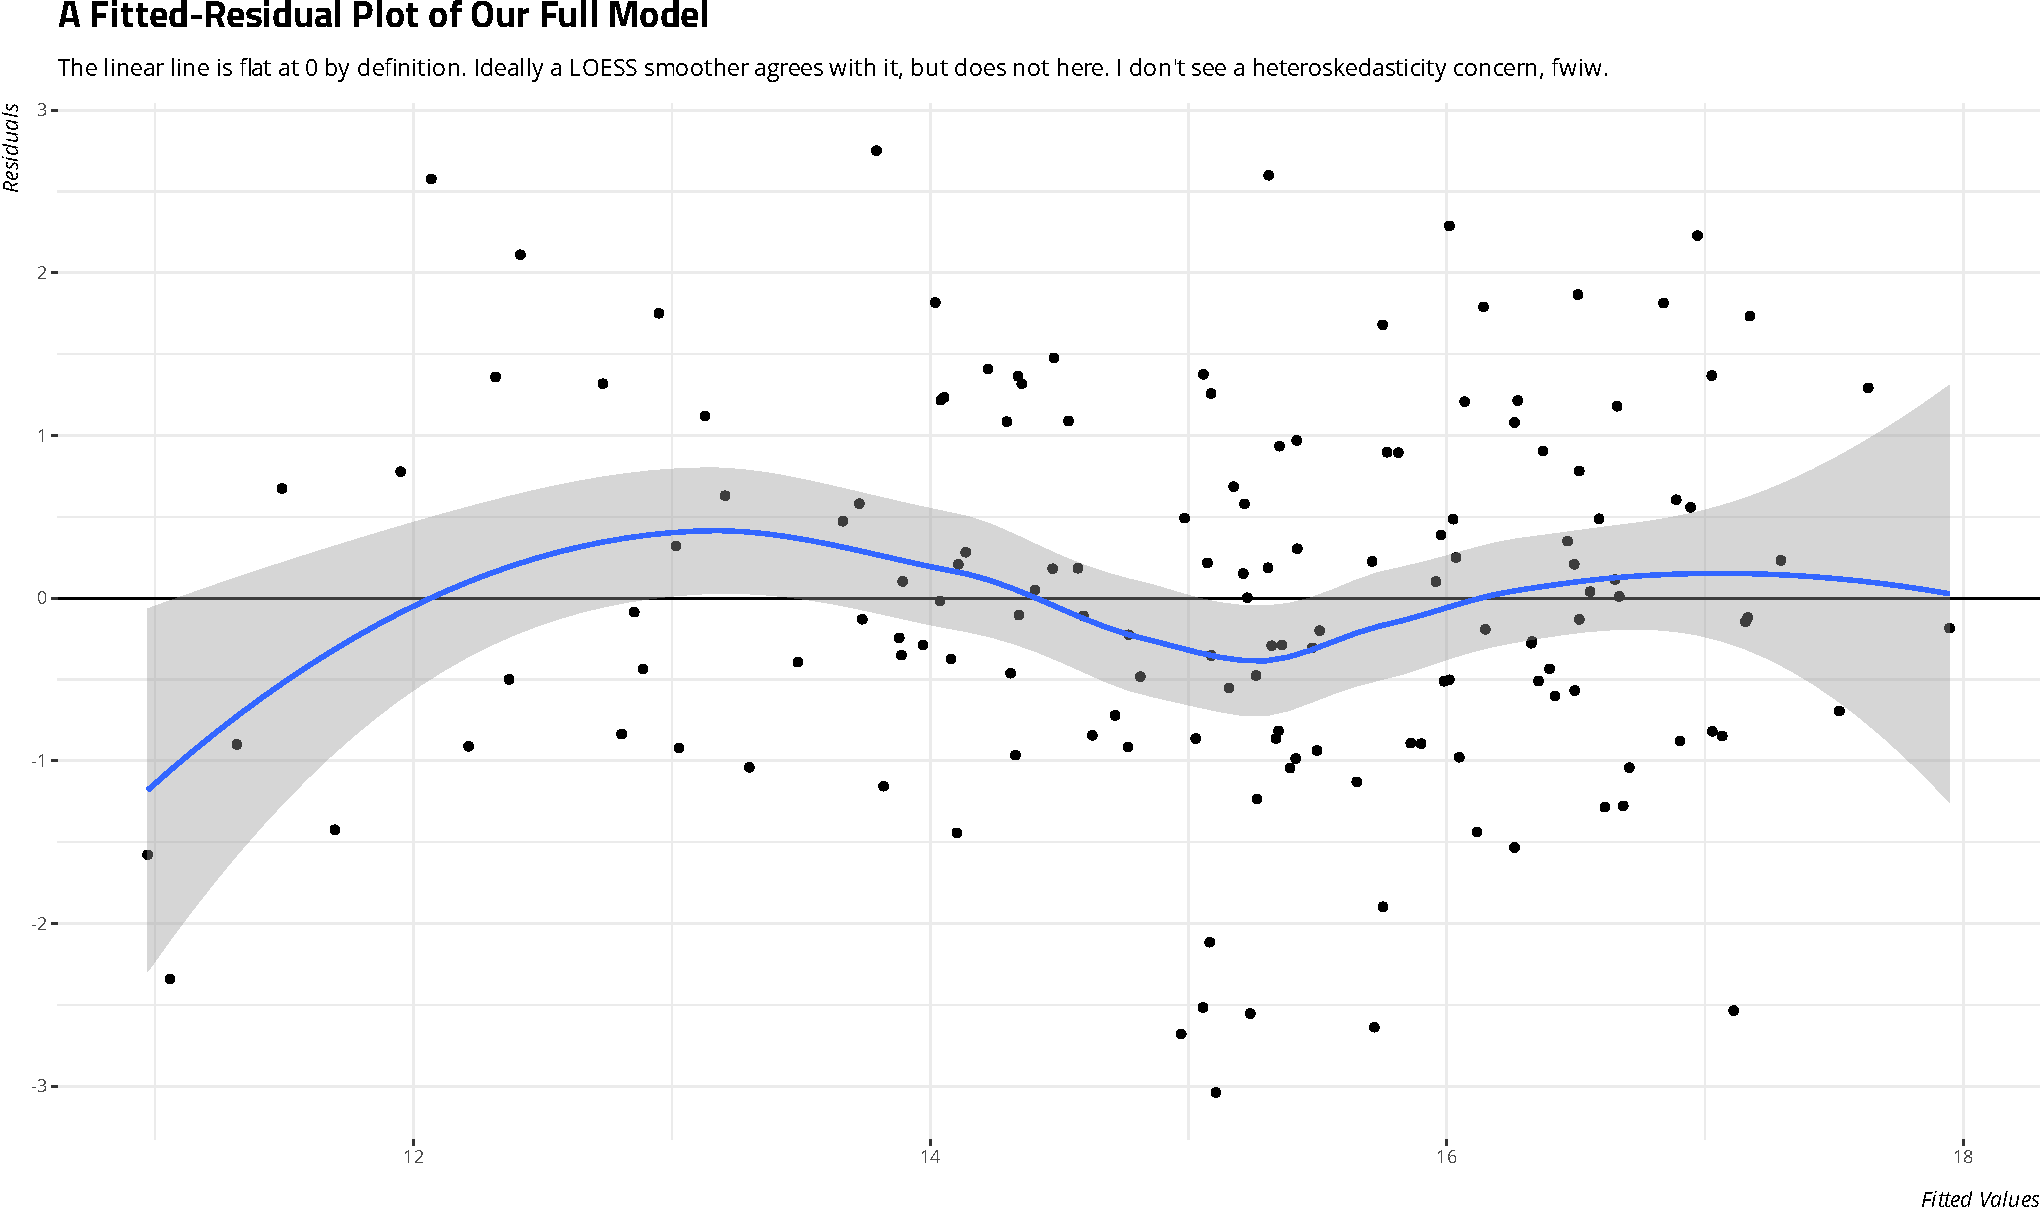
\includegraphics[keepaspectratio]{figs/unnamed-chunk-5.pdf}}
\end{frame}

\begin{frame}{}
\phantomsection\label{section-6}
\pandocbounded{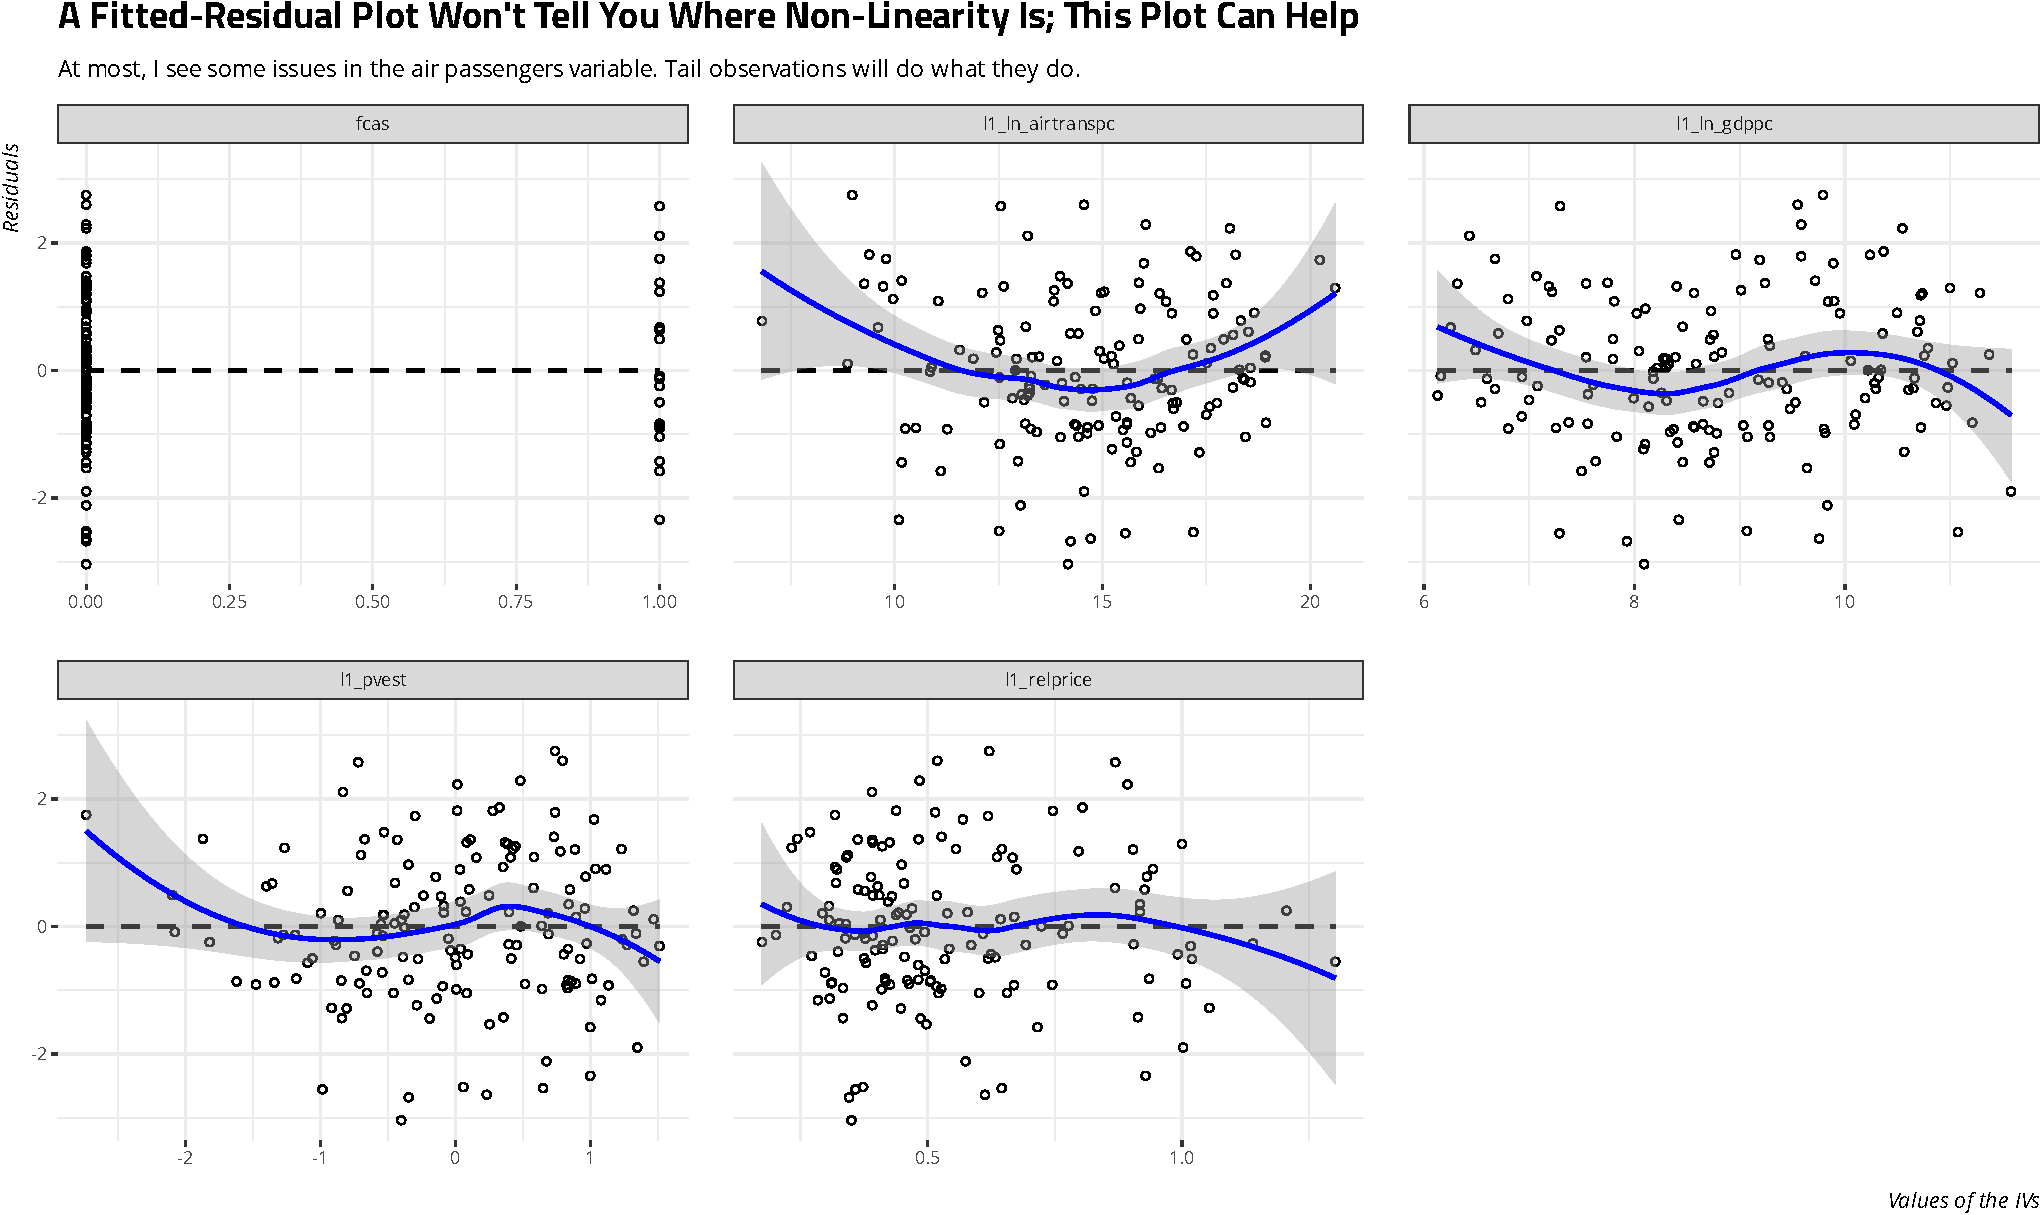
\includegraphics[keepaspectratio]{figs/unnamed-chunk-6.pdf}}
\end{frame}

\begin{frame}{}
\phantomsection\label{section-7}
\pandocbounded{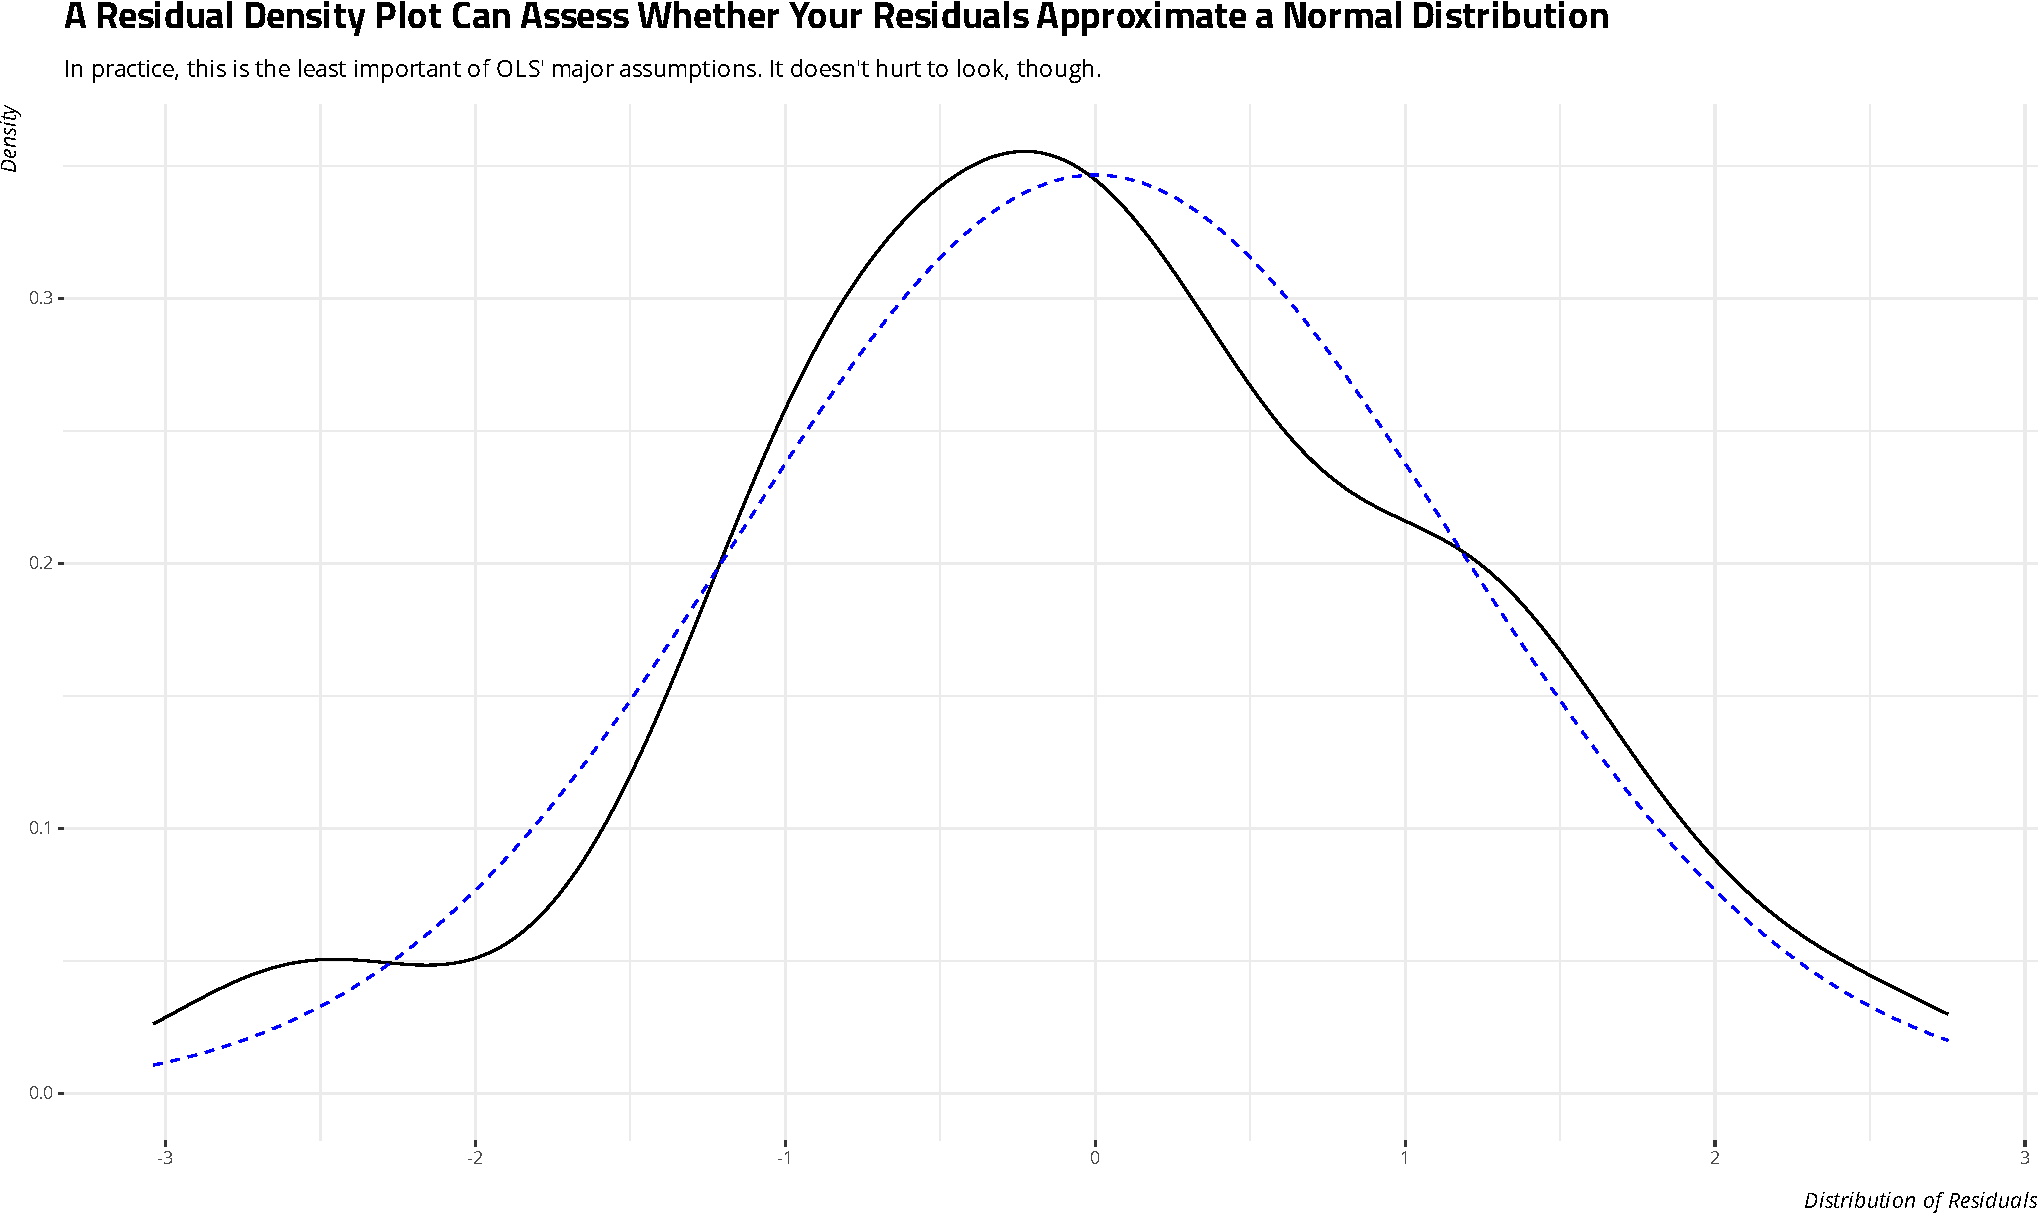
\includegraphics[keepaspectratio]{figs/unnamed-chunk-7.pdf}}
\end{frame}

\section{Conclusion}\label{conclusion}

\begin{frame}{Conclusion}
\phantomsection\label{conclusion-1}
There's \emph{a lot} I crammed into this lecture, but:

\begin{itemize}
\tightlist
\item
  If you remember the slope-intercept equation, the intuition behind
  linear regression isn't much.
\item
  OLS gives you the line of best fit that minimized squared prediction
  errors.
\item
  You gotta get comfortable interpreting regression output.
\item
  Logarithmic transformations proportionalize changes on their raw
  scale.

  \begin{itemize}
  \tightlist
  \item
    This might take some getting used-to, but you should know it.
  \item
    I'll extend grace as you get started, but do wrestle with it.
    Economists definitely do.
  \end{itemize}
\item
  Some parts/assumptions of the linear model are more important than
  others.
\end{itemize}
\end{frame}



\section[]{}
\frame{\small \frametitle{Table of Contents}
\tableofcontents}

\end{document}
